Since we have access to all of the states of the system, we can implement a state feedback control strategy. The control law is given by:
\begin{equation}
    u_k = -\mathbf{K}_x x_k + \mathbf{K}_r \rho_k + \mathbf{K}_u u_{k - 1}
\end{equation}
where $\mathbf{K}_x$ is the state feedback gain matrix, $\mathbf{K}_r$ is the resonant states gain matrix and $\mathbf{K}_u$ is the previous control input gain matrix.

\begin{figure}[t!]
    \centering
    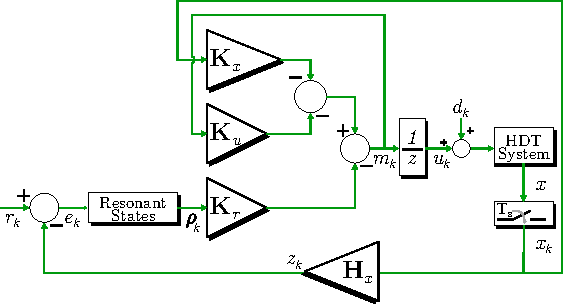
\includegraphics[width=\columnwidth]{Images/Control_Diagram.pdf} 
    \caption{Block diagram of the proposed control strategy for the HDT.}
    \label{fig:Control_Diagram}
\end{figure}

The resonant states are included to ensure zero steady-state error for sinusoidal references and disturbances. The resonant states dynamics are given by:
\begin{equation}
    \dfrac{d\,\rho(t)}{dt} = 
    \underbrace{
    \begin{bmatrix}
        -\xi\omega & \omega \\
        -\omega & \xi\omega
    \end{bmatrix}
    }_{\mathbf{A}_r}
    \rho(t) + 
    \underbrace{
    \begin{bmatrix}
        1\\
        0
    \end{bmatrix}
    }_{\mathbf{B}_r}
    e(t)
\end{equation}
where $\omega$ is the nominal angular frequency, $\xi$ is the damping factor, and $e(t)$ is the error signal defined as the difference between the reference and the measured output. Each of the references signals has two resonant states associated with it, meaning that for the HDT control, there are eight resonant states in total (4 for the $ev_{cs,\alpha\beta}$ and 4 for the $i_{fp,\alpha\beta}$). This can be expressed as:
\begin{align}
    \dfrac{d\,\rho(t)}{dt} &= \text{blkdiag}(\mathbf{A}_r, \mathbf{A}_r, \mathbf{A}_r, \mathbf{A}_r)\rho(t)\\
    &+ \text{blkdiag}(\mathbf{B}_r, \mathbf{B}_r, \mathbf{B}_r, \mathbf{B}_r)e(t)
\end{align}

The augmented state-space model of the HDT can be expressed as:
\begin{align}
    \begin{aligned}
        \dfrac{d}{dt}
        \begin{bmatrix}
            x\\
            \rho
        \end{bmatrix}
        &=
        \begin{bmatrix}
            \mathbf{A} & \mathbf{0} \\
            \mathbf{B}_r\mathbf{H} & \mathbf{A}_r
        \end{bmatrix}
        \begin{bmatrix}
            x\\
            \rho
        \end{bmatrix}
        +
        \begin{bmatrix}
            \mathbf{B}_{d,\text{aug}}\\
            \mathbf{0}
        \end{bmatrix}
        \begin{bmatrix}
            u\\
            e
        \end{bmatrix}
        \\
        y &= 
        \begin{bmatrix}
            \mathbf{C} & \mathbf{0}
        \end{bmatrix}
        \begin{bmatrix}
            x\\
            \rho
        \end{bmatrix}
    \end{aligned}
\end{align}

\subsection{Particle Swarm Optimization}

The PSO algorithm is a population-based optimization technique inspired by the social behavior of birds and fish. It consists of a swarm of particles, where each particle represents a potential solution to the optimization problem. The particles move through the search space, updating their positions based on their own experience and the experience of their neighbors. The velocity and position of each particle are updated using the following equations:
\begin{align}
    \begin{aligned}
        v_j(i + 1) &= K_{ap}\left(v_j(i) + c_1 r_1 (pbest_j - x_j(i)) \right.\\
        & \left. + c_2 r_2 (gbest - x_j(i))\right)\\
        x_j(i + 1) &= x_j(i) + v_j(i + 1)
    \end{aligned}
\end{align}
where $v_j(i)$ is the velocity of particle $j$ at iteration $i$, $x_j(i)$ is the position of particle $j$ at iteration $i$, $pbest_j$ is the best position found by particle $j$, $gbest$ is the best position found by the entire swarm, $c_1$ and $c_2$ are cognitive and social acceleration coefficients, $r_1$ and $r_2$ are random numbers uniformly distributed in the range [0, 1], and $K_{ap}$ is the constriction factor given by:
\begin{equation}
    K_{ap} = \dfrac{2}{\left|2 - \phi - \sqrt{\phi^2 - 4\phi}\right|}
\end{equation}
where $\phi = c_1 + c_2 > 4$ is a constant that ensures convergence.

The PSO algorithm iteratively updates the positions and velocities of the particles until a stopping criterion is met, such as a maximum number of iterations or a satisfactory solution. The best position found by the swarm is considered the optimal solution to the optimization problem.